% !TEX root = ../paper.tex
%
% ---------- chapter 5 ----------
%
% define project name notation
\newcommand{\projectA}[0]{\emph{A-Input}}
\newcommand{\projectB}[0]{\emph{B-DBUpgrade}}
\newcommand{\projectC}[0]{\emph{C-SmartPrice}}

  \vspace{-2mm}
\section{Experimental Results}
  \vspace{-2mm}
To assess the evolutionary algorithm proposed in this paper, two separated
evaluation experiments are made for the effectiveness of evolutionary algorithm
and the efficiency of parallel evolutionary algorithm in project management
problem. The purpose of the experiment is to address the following two
research questions:

\textbf{RQ1}: Does the evolutionary algorithm effectively optimize project
management problem, and get an optimized solution?

\textbf{RQ2}: Is the parallel evolutionary algorithm able to improve the
efficiency in the project management problem?

  \vspace{-2mm}
\subsection{Industrial Project Data}
%
Three industrial project plans have been used in the experimental studies for
this paper, which are named as \projectA{}, \projectB{} and \projectC{}. These
data come from real world projects and have fundamental details, such as work
packages, resources and dependencies. Table \ref{tab:statis} shows the number of
each project.

% 
\begin{table}[!h]
\vspace{-6mm}
  \centering
  \caption{Three Project's Parameters}
        \vspace{-2mm}
  \label{tab:statis}
  \begin{tabular}{lccc}
    \hline
      & $\#$ work packages & $\#$ resources & $\#$ dependencies \\
    \hline
    \projectA{} & 33  & 4  & 33  \\
    \projectB{} & 106 & 8  & 105 \\
    \projectC{} & 74  & 14 & 73  \\
    \hline
  \end{tabular}
  \vspace{-6mm}
\end{table}

\projectA{} is a simulated small-scale project planning. it is a team work plan
for finishing class assignments. \projectB{} is a real software development
plan, which's goal is to upgrade the Oracle database from the \emph{9g} version
to the \emph{10g} version. \projectB{} is Oracle's non-public version of the
project planning. There were different layers of the organisation involved
including DBAs, BSAs, developers and users.  Furthermore, the project also
included the training of the staff for the new features of the
system. \projectC{} consists of a supply chain enhancement of medium size
affecting mostly the website as well as a few internal applications~\cite{ren2}.

Figure \ref{fig:dag} illustrates the relationship between work packages and
resources. In each sub-figure, the rectangle represents a work package in the
project plan, the content in the rectangle is the work packages' ID and
duration; the arrows between work packages suggest dependencies, notice that
some redundant dependencies is removed; the folders in the bottom are some
certain types of resources that can be allocated to work packages. 

\begin{figure}[!ht]
  \centering
  \subfigure[\projectA{}, $33$ work packages, $4$ resources and $33$ dependencies]{
    \centering
    \label{fig:dag:a} 
    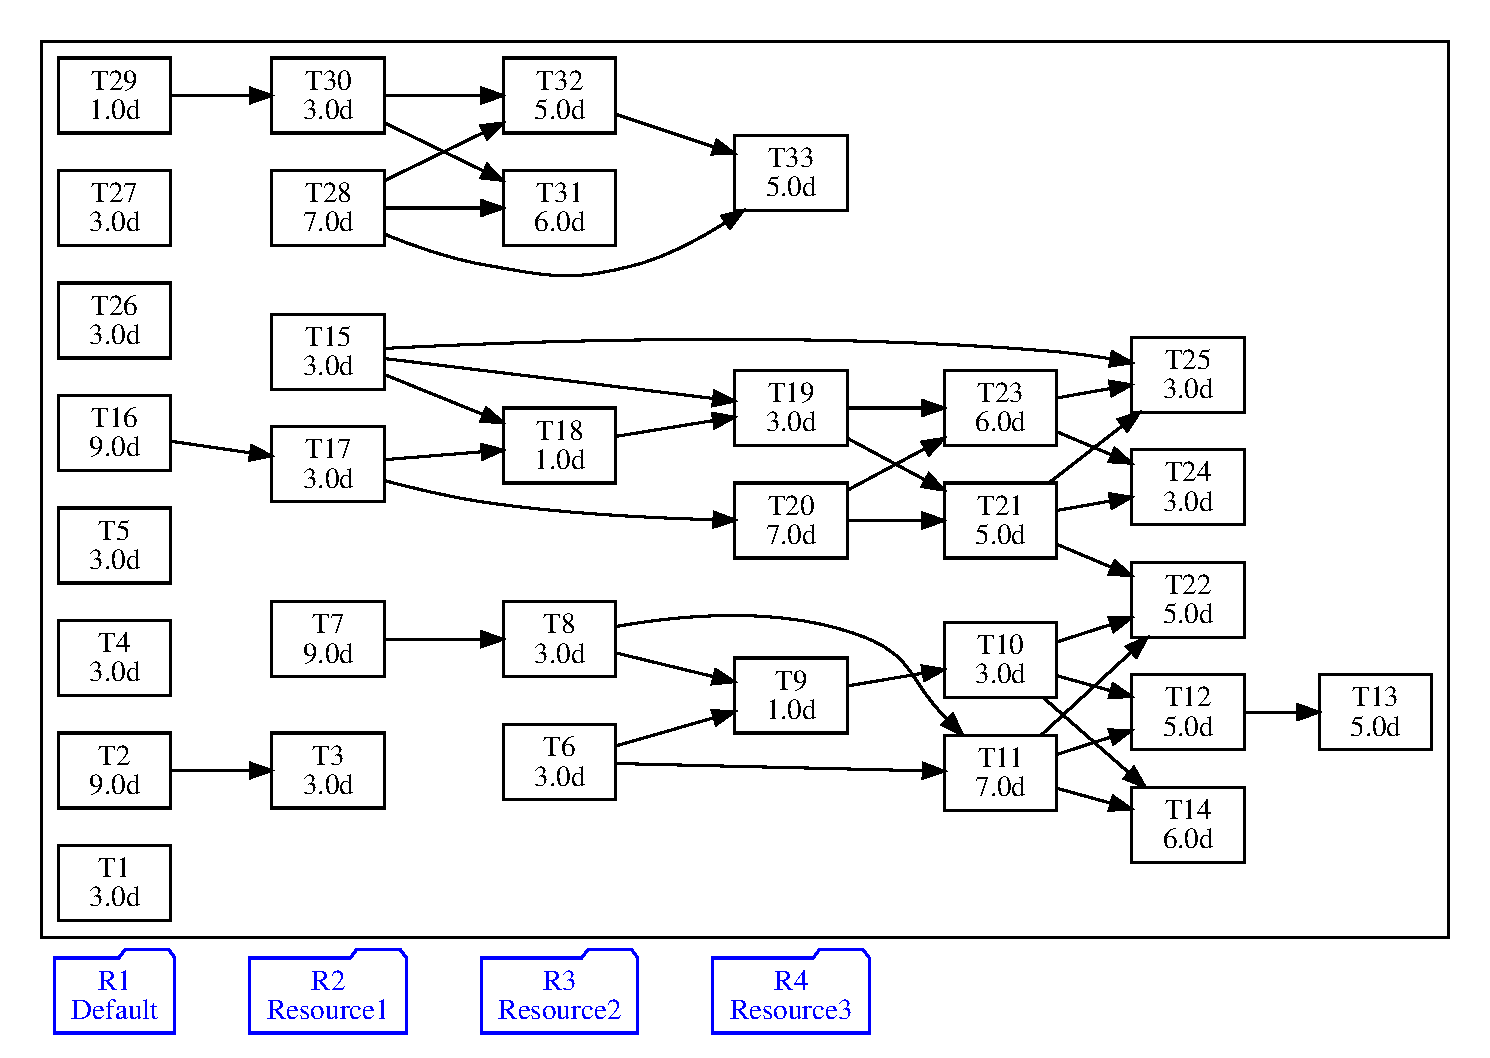
\includegraphics[width=0.75\textwidth]{figures/a.eps}
  }
  \subfigure[\projectB{}: $106$ work packages, $8$ resources and $105$ dependencies]{
    \centering
    \label{fig:dag:b}
    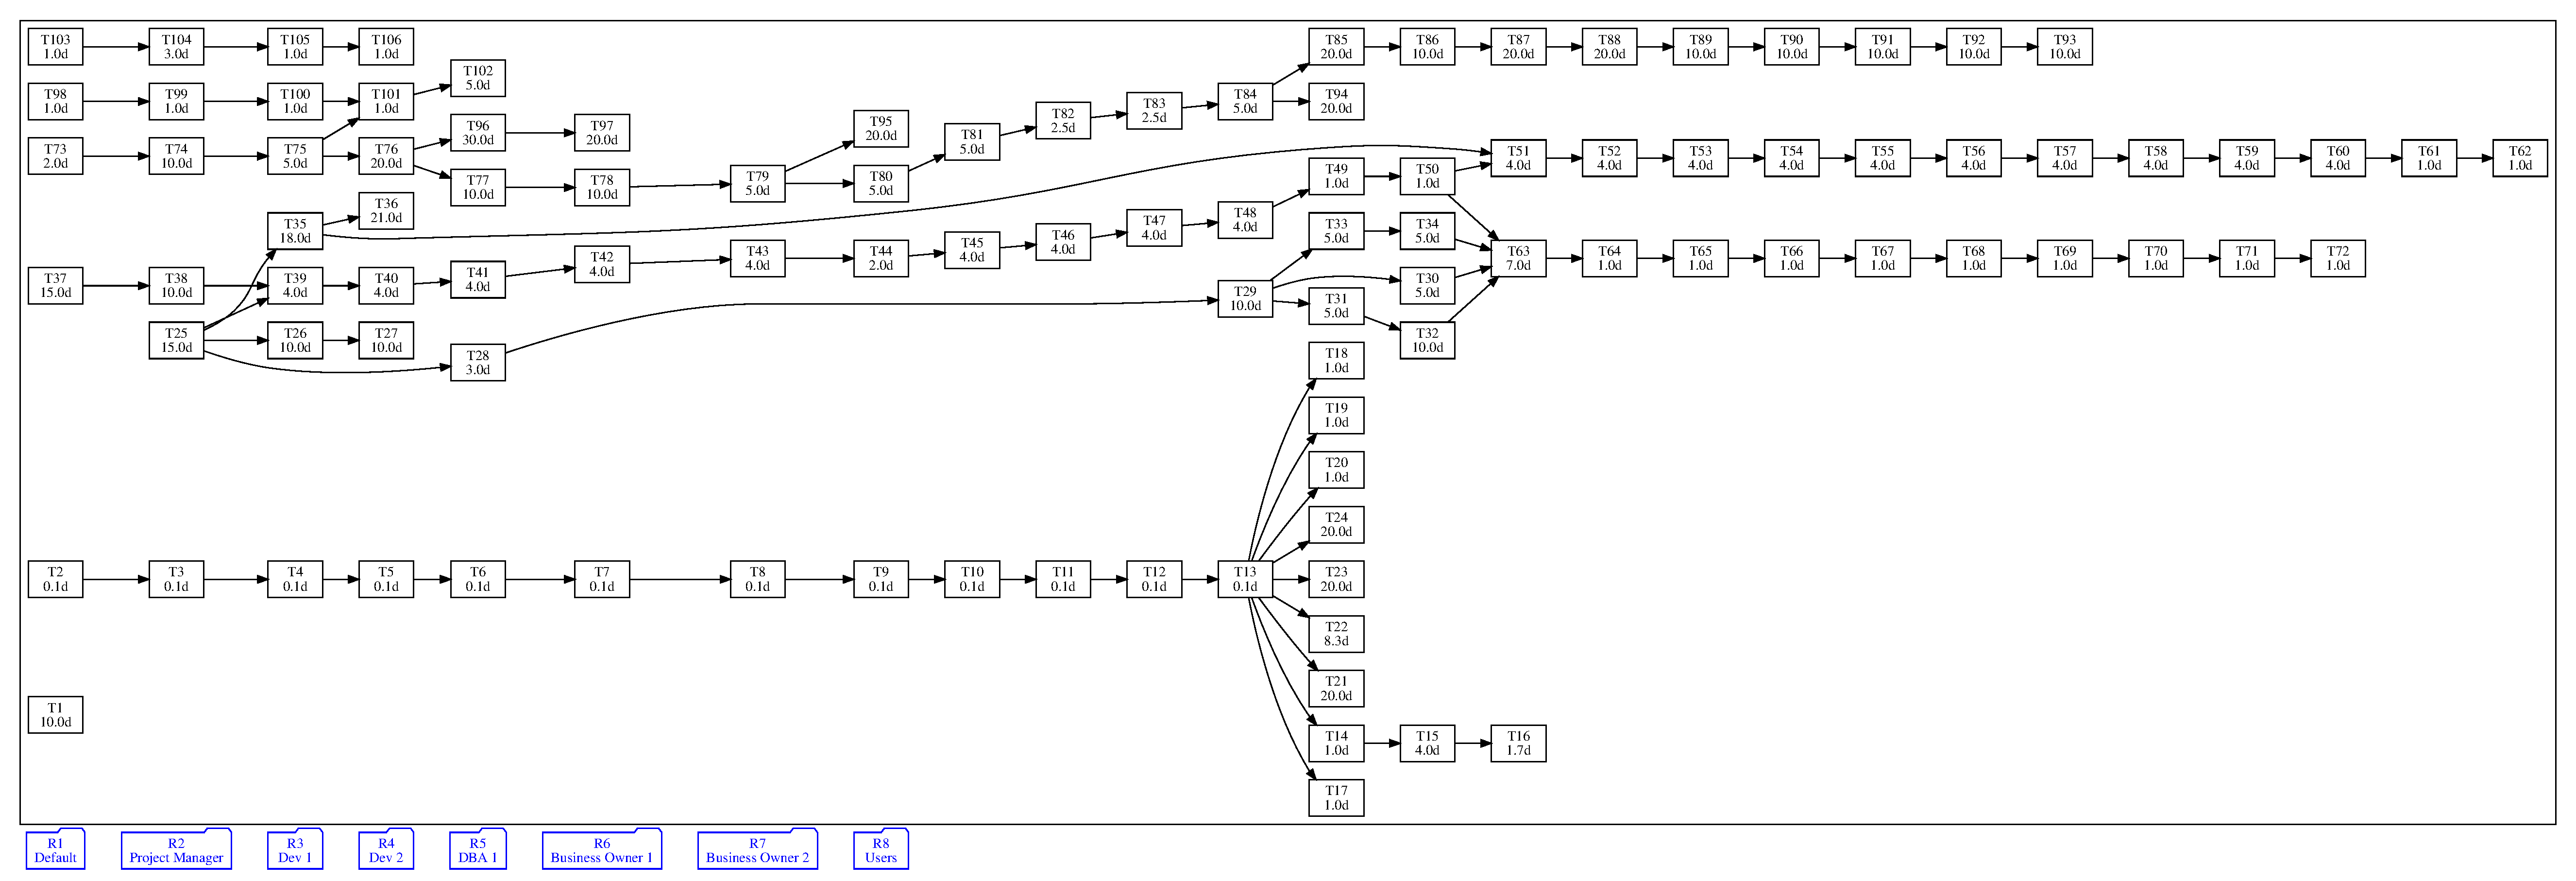
\includegraphics[width=\textwidth]{figures/b.eps}
  }
  \subfigure[\projectC{}:, $74$ work packages, $14$ resources and $73$ dependencies]{
    \centering
    \label{fig:dag:c}
    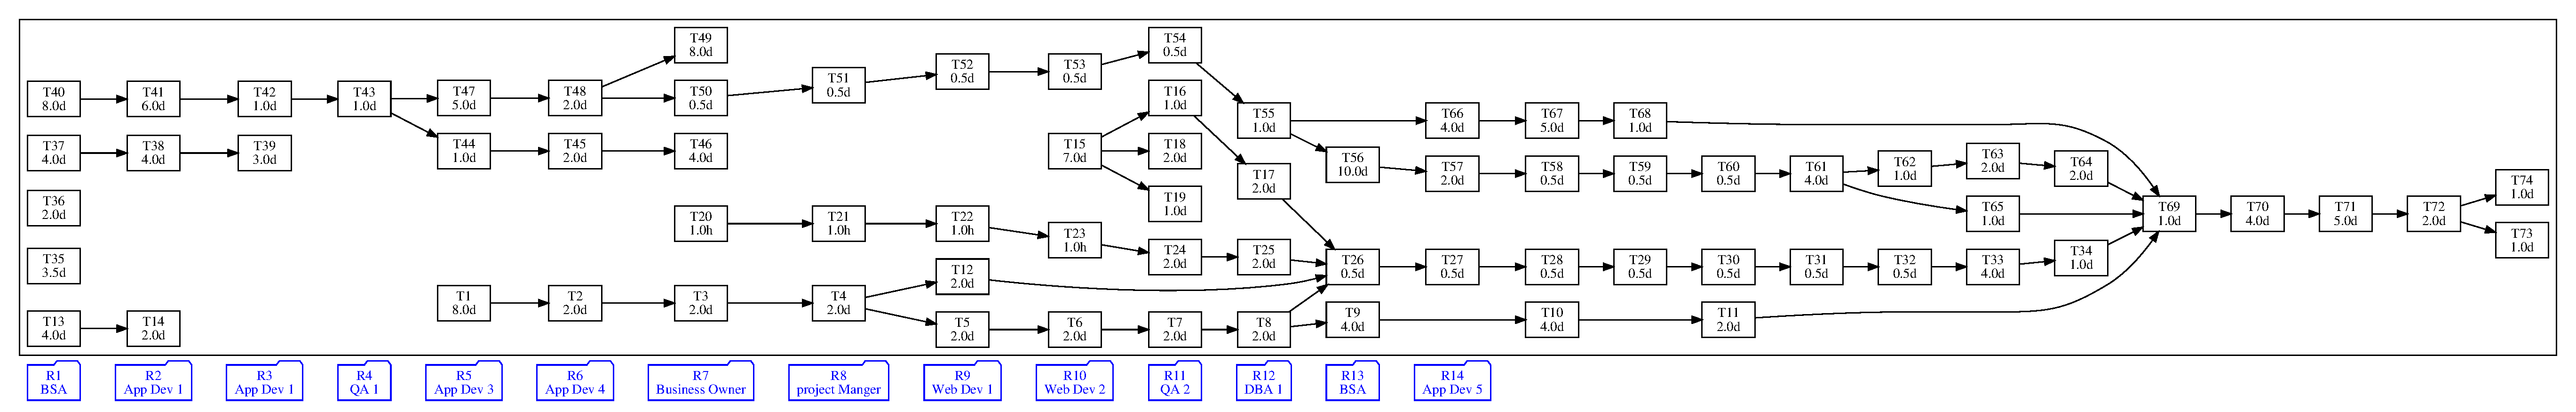
\includegraphics[width=\textwidth]{figures/c.eps}
  }
        \vspace{-5mm}
  \caption{Three Projects' \emph{work packages}, \emph{resources} and \emph{dependencies}}
  \label{fig:dag}
  \vspace{-5mm}
\end{figure}


\subsection{Effectiveness Experiment for Algorithm}
%
In order to answer \textbf{RQ1}, this section designs an effectiveness experiment
for evolutionary algorithm. The basic configuration used in the experiment is
that $100$ individuals runs in $50$ generations. For each generation in the
evolutionary algorithm, we evaluate each individuals' fitness value in the
whole population, and then plot the statistical data into a boxplot diagram.

% effectiveness experiment results
\begin{figure}[!h]
  \centering
        \vspace{-2mm}
  \subfigure[\projectA{}'s solution converges on \emph{19th} generation]{
    \label{fig:pj:a} 
    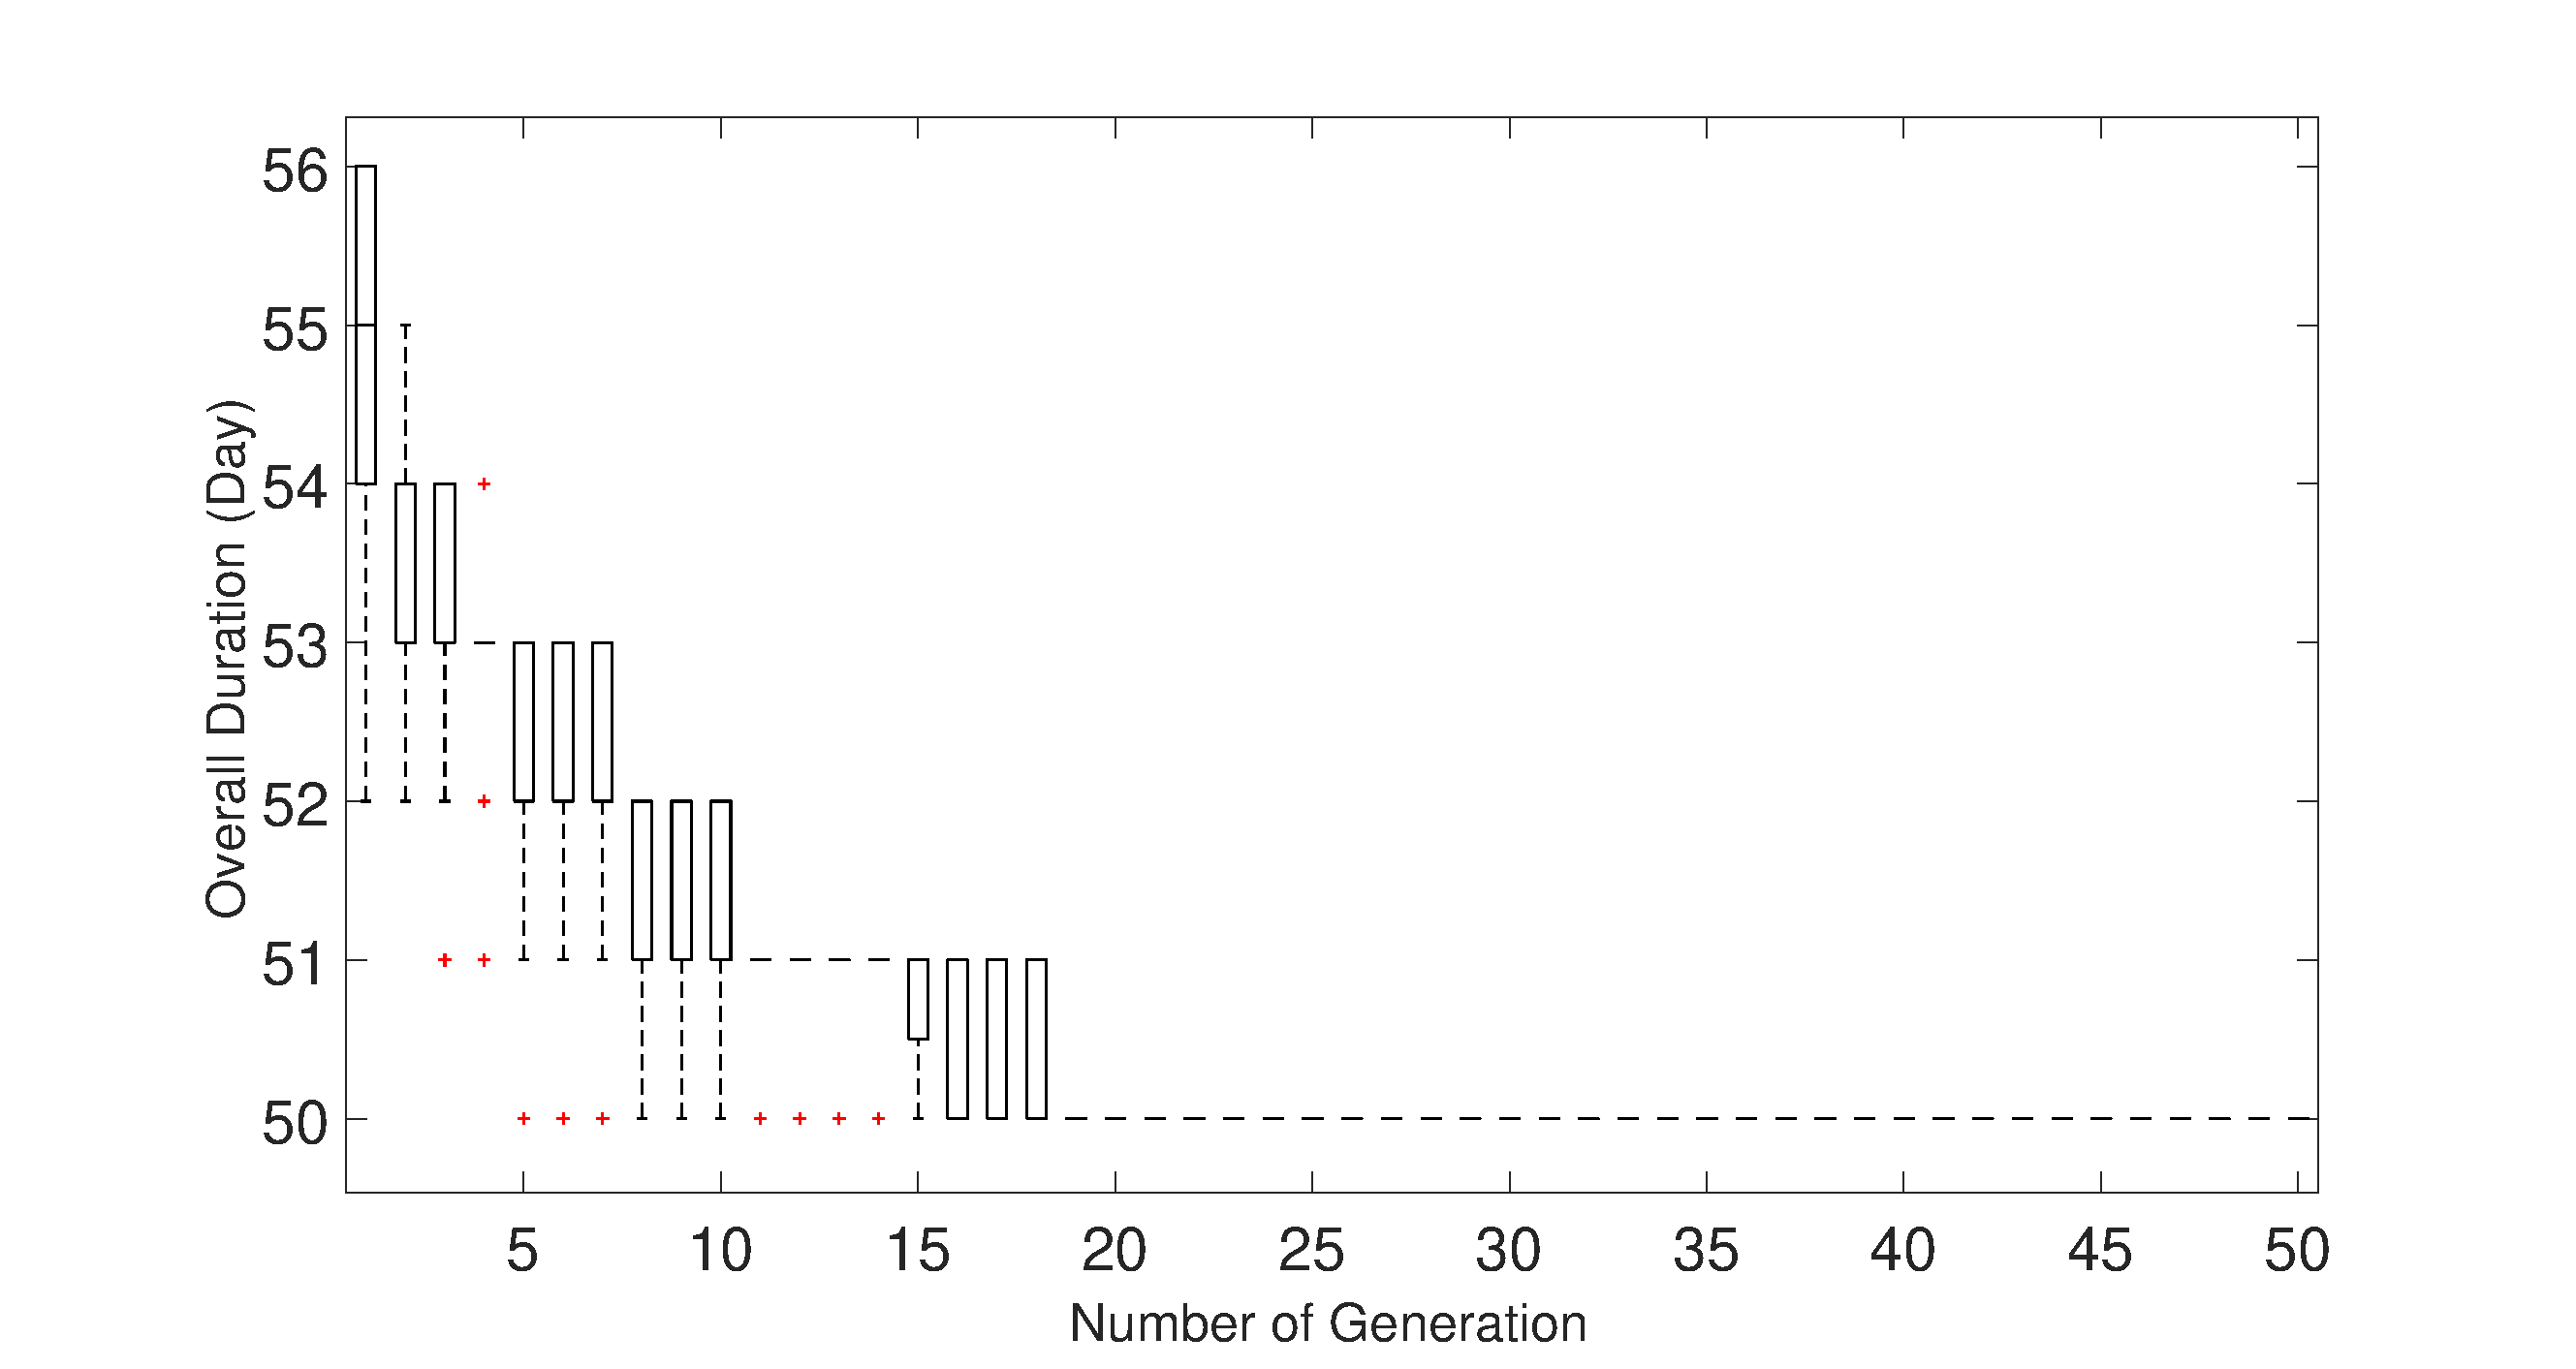
\includegraphics[width=.7\textwidth]{figures/fig_pa1.eps}
  }
      \vspace{-2mm}
  \subfigure[\projectB{}'s solution converges on \emph{22rd} generation]{
    \label{fig:pj:b} 
    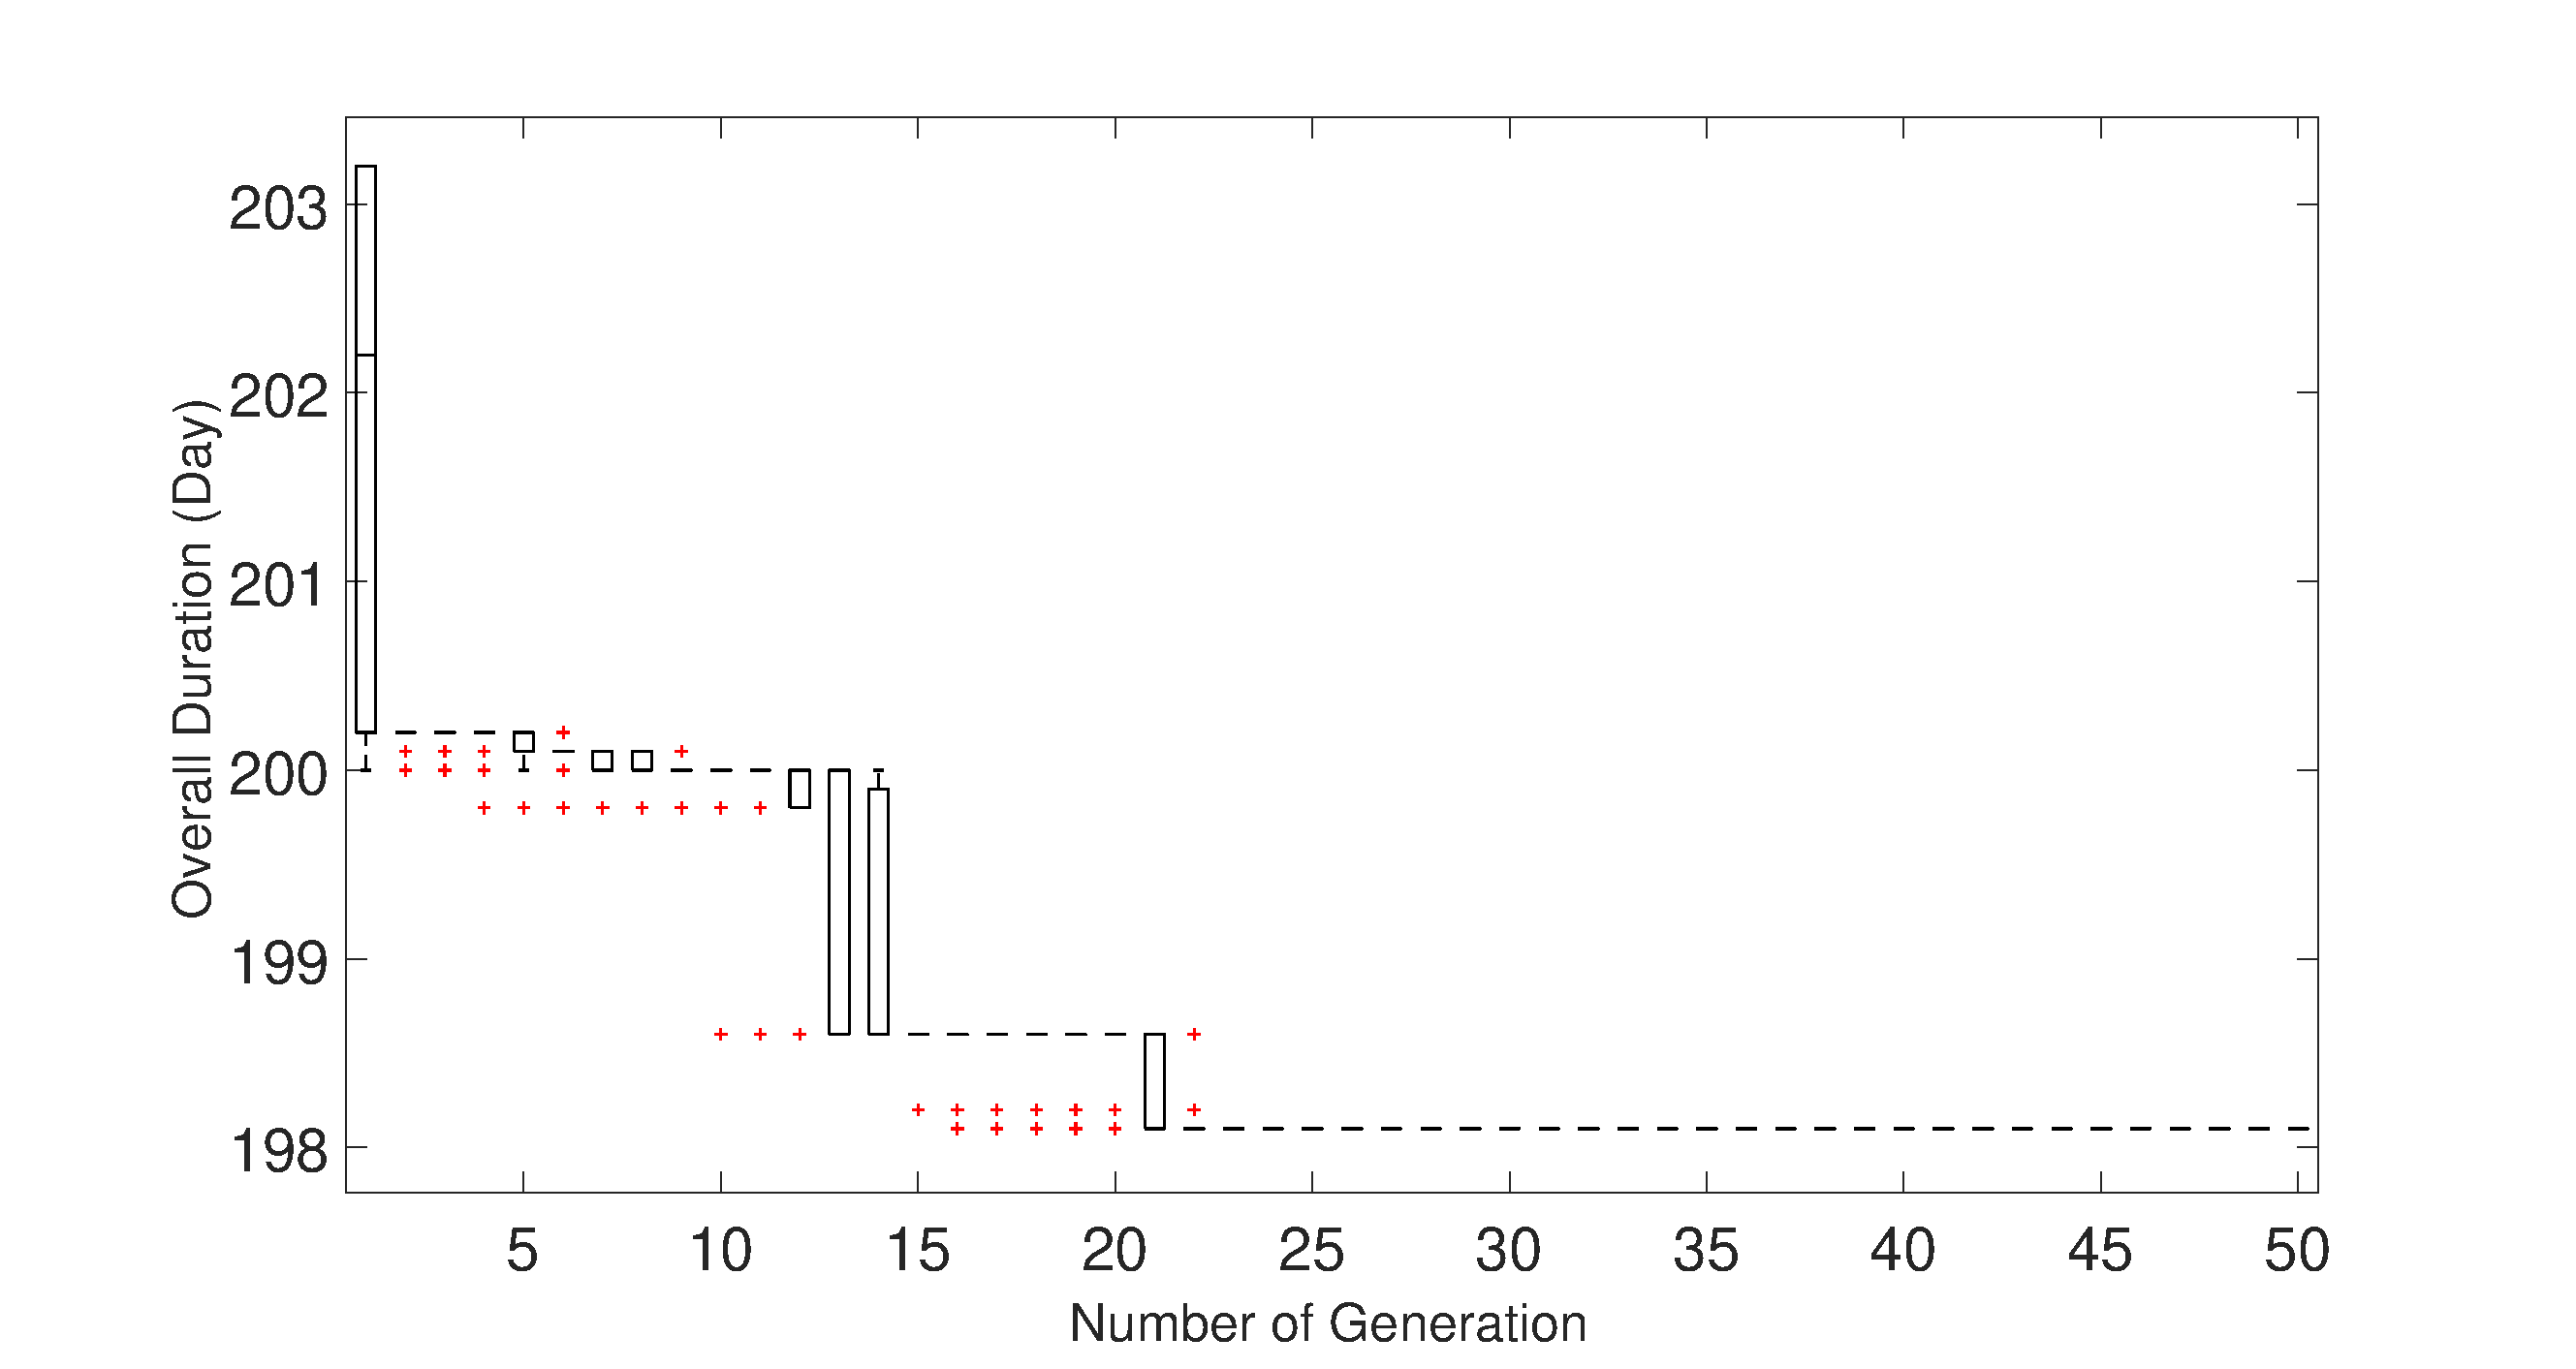
\includegraphics[width=.7\textwidth]{figures/fig_pa2.eps}
  }
        \vspace{-2mm}
  \subfigure[\projectC{}'s solution converges on \emph{15th} generation]{
    \label{fig:pj:c} 
    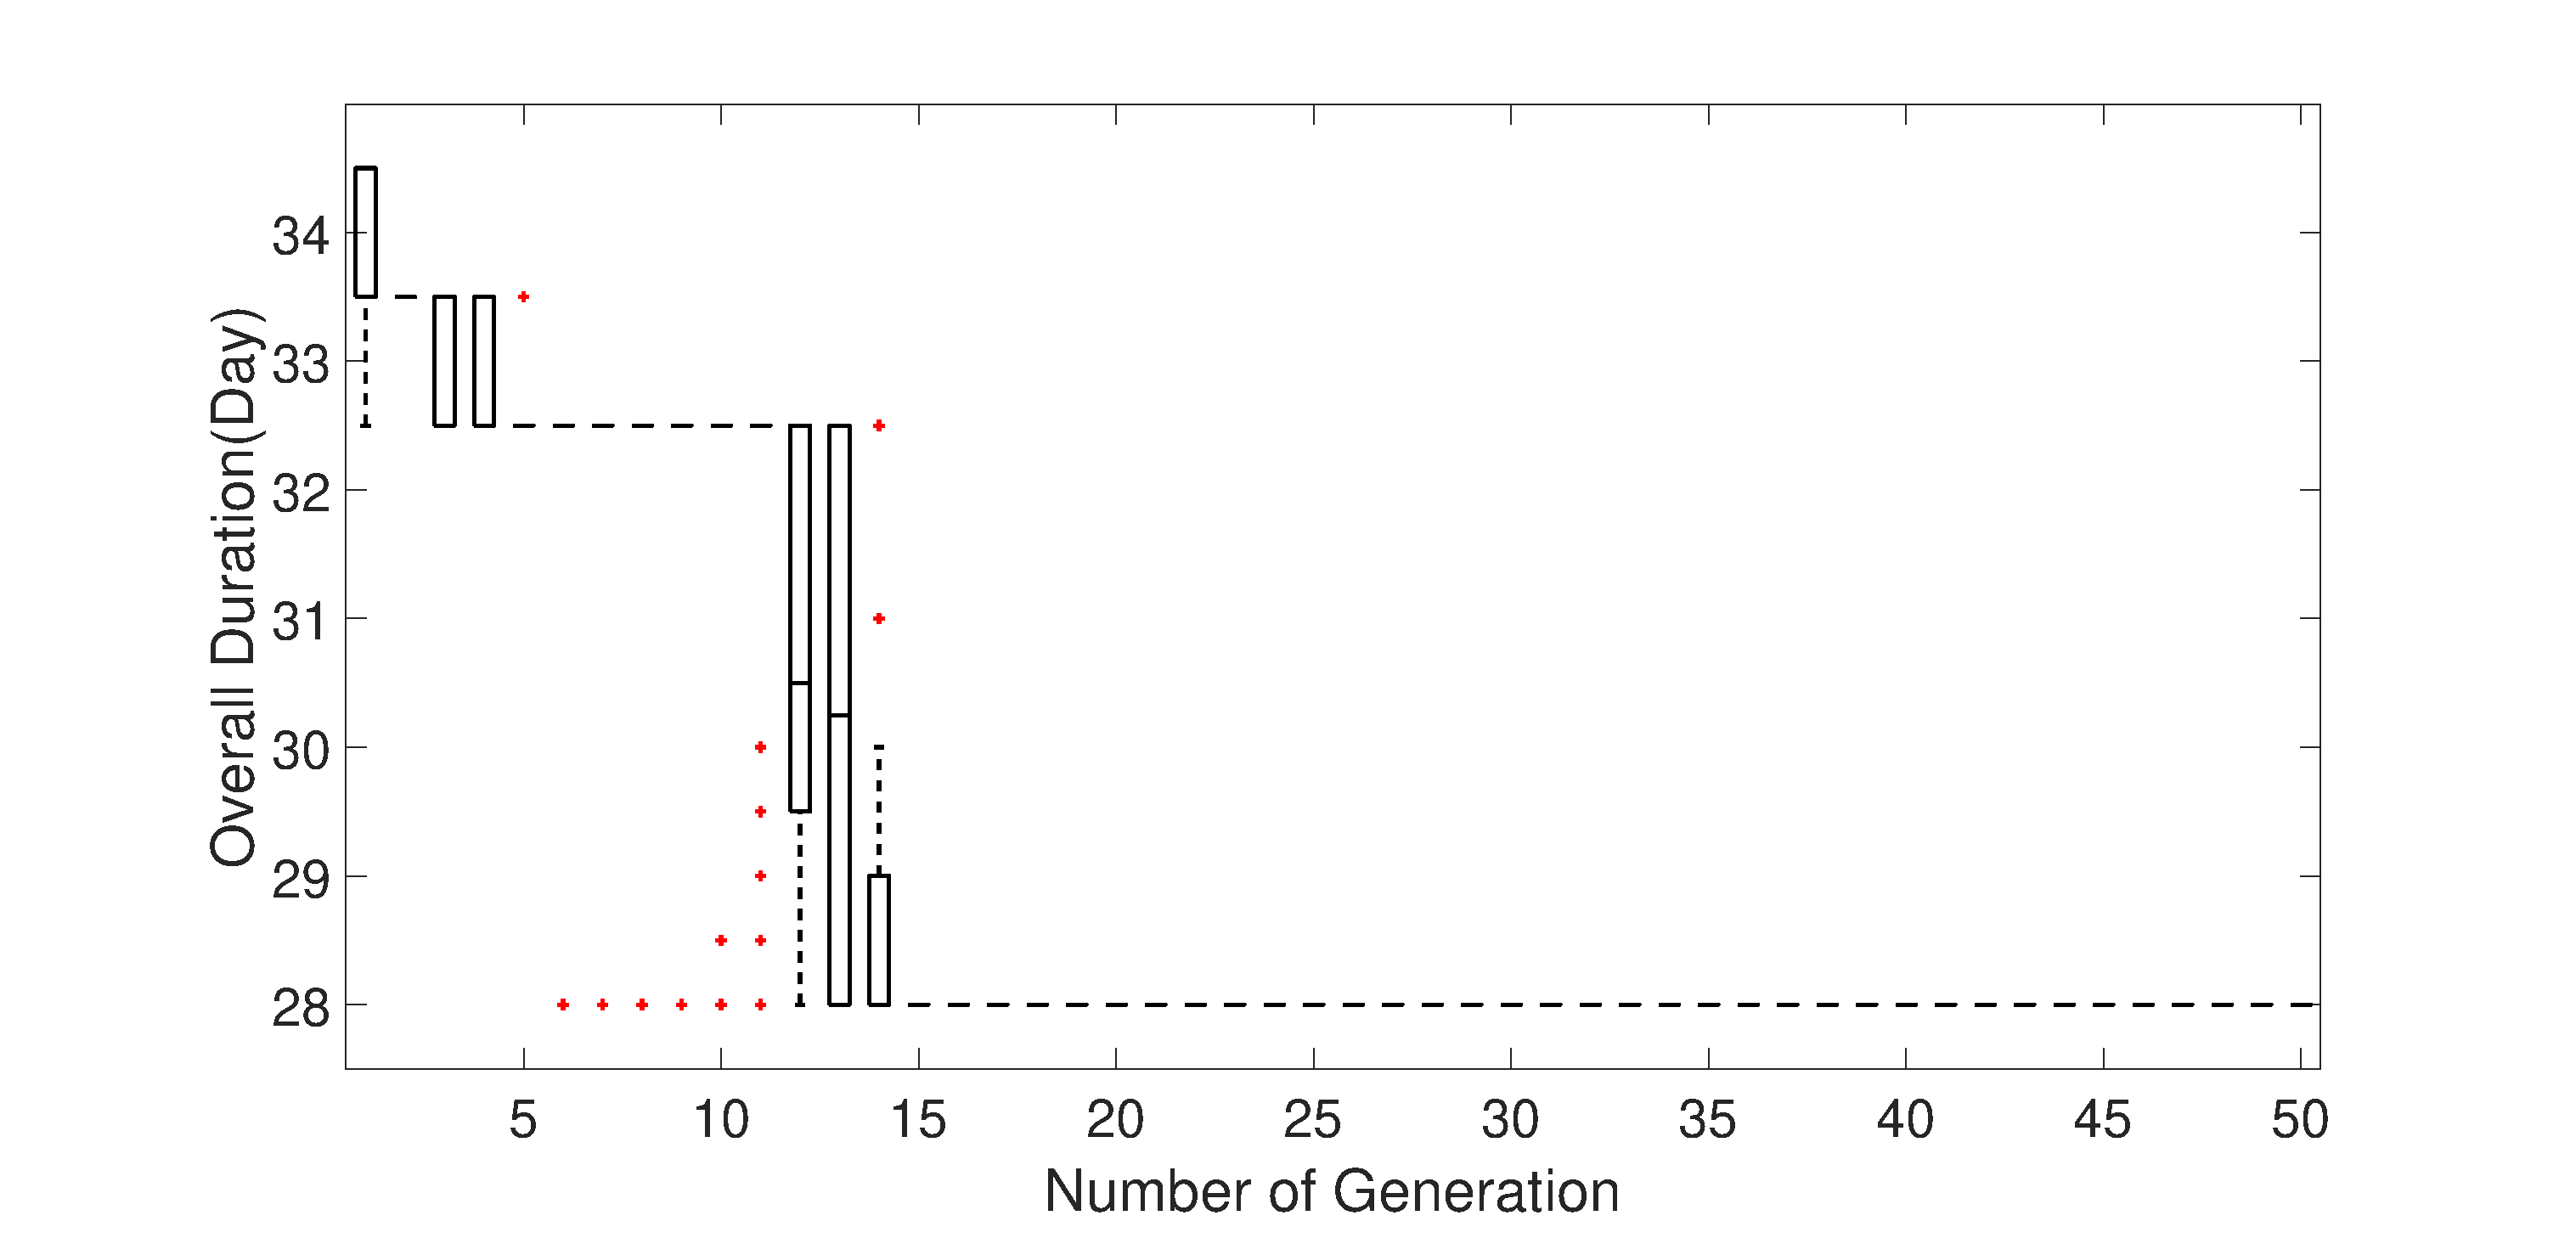
\includegraphics[width=0.7\textwidth]{figures/fig_pa3.eps}
  }
  \caption{Statistics of Fitness Value in Each Generation}
  \label{fig:pj}
  \vspace{-8mm}
\end{figure}

The boxplot diagram shows the five kinds of statistical data of all individuals'
fitness value in each generation. The data are the minimum, the lower quartile,
the median, the upper quartile and the maximum values of the whole
population. Figure \ref{fig:pj} shows the results of the above-mentioned three
industrial projects. In each sub-figure, the tick labels on the horizontal axis
indicate the total number of internal generations that have been carried out,
and also indicates the point at which the algorithm updated the population used
for fitness computation. At each point on the horizontal axis, the entire
population is depicted using a boxplot to give both a sense of the values
obtained for completion time as the evolution progresses and the distribution of
the fitness values in the population. From the trend of three projects in the
figures, it can be seen that the population is diversified when the population
is initialized and as the number of generation increase, all the fitness value
begins to decrease, and finally converges to an optimized result.

The convergence of solutions is quite fast and stable. Figure \ref{fig:pj:a}
shows the solution of \projectA{} converges on 19th generation. Figure
\ref{fig:pj:b} shows the solution of \projectB{} converges on 22rd generation.
Figure \ref{fig:pj:c} shows the solution of \projectC{} converges on 15th
generation. Those results show us evolutionary algorithm will find an optimized
overall duration for specific project plan.

Through the above analysis results of experimental data, we can accurately
answer \textbf{RQ1}. In the project management problems, the evolutionary
algorithm does have a good optimization and improvement.


\subsection{Efficiency Experiment for Algorithm}
%
In order to answer \textbf{RQ2}, this section conducts an efficiency experiment
that compares the efficiency between the parallel evolutionary algorithm and the
sequential one.

%% \begin{table}[!ht]
%%   \centering
%%   \caption{Hardware Configuration Comparison}
%%   \label{tab:cpugpu}
%%   \begin{tabular}{c|c}
%%     \hline
%%     CPU & GPU  \\
%%     \hline
%%     \hspace{.5cm} Intel i7 CPU 870 \hspace{.5cm} & \hspace{.5cm} GeForce GTX 970 \hspace{.5cm} \\
%%     2.93 GHz & 1.27 GHz \\
%%     8 cores & 1664 cores \\
%%     \hline
%%   \end{tabular}
%% \end{table}

\begin{table}[!h]
\vspace{-7mm}
  \centering
  \caption{The Comparison of Sequential and Parallel Implementation}
  \vspace{-3mm}
  \label{tab:time}
  \begin{tabular}{ccc|cc|cc}
    \hline
    & \multicolumn{2}{c}{ \projectA{} } & \multicolumn{2}{c}{ \projectB{} } & \multicolumn{2}{c}{ \projectC } \\
    \hline
      Time(ms) & \hspace{.25cm} CPU \hspace{.25cm} & \hspace{.25cm} GPU \hspace{.25cm} & \hspace{.25cm} CPU \hspace{.25cm} & \hspace{.25cm} GPU \hspace{.25cm} & \hspace{.25cm} CPU \hspace{.25cm} & \hspace{.25cm} GPU \hspace{.25cm}\\
    \hline
     1    & 7991.8 & 4102.5 & 45225.1 & 21217.5 & 29642.9 & 14844.3 \\
     2    & 8431.8 & 4279.7 & 44832.1 & 21377.9 & 28733.7 & 14543.6 \\
     3    & 7504.1 & 3947.9 & 44934.9 & 21227.2 & 28657.9 & 15003.4 \\
     4    & 7442.1 & 4642.5 & 44197.1 & 21340.3 & 29489.5 & 14882.8 \\
     5    & 7376.9 & 4263.8 & 45233.7 & 22448.2 & 29379.5 & 14921.5 \\
     6    & 7385.4 & 4188.6 & 45197.5 & 20956.1 & 28687.9 & 14723.3 \\
     7    & 8238.8 & 4540.2 & 45305.4 & 21777.2 & 29786.3 & 13978.8 \\
     8    & 7470.7 & 4226.4 & 45322.8 & 21147.1 & 31231.7 & 14811.1 \\
     9    & 7604.8 & 3778.2 & 45040.7 & 21004.7 & 28319.7 & 14292.0 \\
     10   & 7451.9 & 4712.4 & 45970.6 & 21500.9 & 28322.1 & 14429.7 \\
    \hline
     Avg. & 7689.8 & 4268.2 & 45126.0 & 21399.7 & 29225.1 & 14643.1 \\
    \hline
  \end{tabular}
  \vspace{-7mm}
\end{table}


The initial configuration of the two algorithms is the identical, which the
number of population is $1000$ and the number of generation is $100$. Each
generation runs several steps including crossover, mutation and selection etc. A
timer is set to record the total executing time of the experiments. The timer
starts after loading initial data and ends after the result is calculated. This
operation allows us to count the real executing time both in the sequential
environment and the parallel environment under the same criteria. The efficiency
experiments are repeated $10$ times. Table \ref{tab:time} shows the comparison
of sequential and parallel implementation executing time on all three industrial
projects. By the comparison of average executing time of $10$ times results, the
average executing time of \projectA{} on CPU is $1.80$ times than GPU, the
average executing time of \projectB{} on CPU is $2.10$ times than GPU and the
average executing time of \projectC{} on CPU is $2.00$ times than GPU.

In summary, the executing time of sequential algorithm on CPU is roughly twice
as long as the parallel algorithm on GPU. So it can be a good answer to
\textbf{RQ2} that parallel evolutionary algorithm can improve the efficiency on
computing the project management problems.

%% The final result of \projectA{}, \projectB{} and \projectC{} are
%% shown in figures \ref{fig:co}. It can be seen from the figures that the
%% time-consuming of the sequential algorithm on CPU is roughly twice as long as
%% the parallel algorithm on GPU.


% comparison figures
%% \begin{figure}[!hb]
%%   \centering
%%   \subfigure[\projectA{}'s executing time spend on CPU is \emph{1.80} times than GPU]{
%%     \label{fig:co:a}
%%     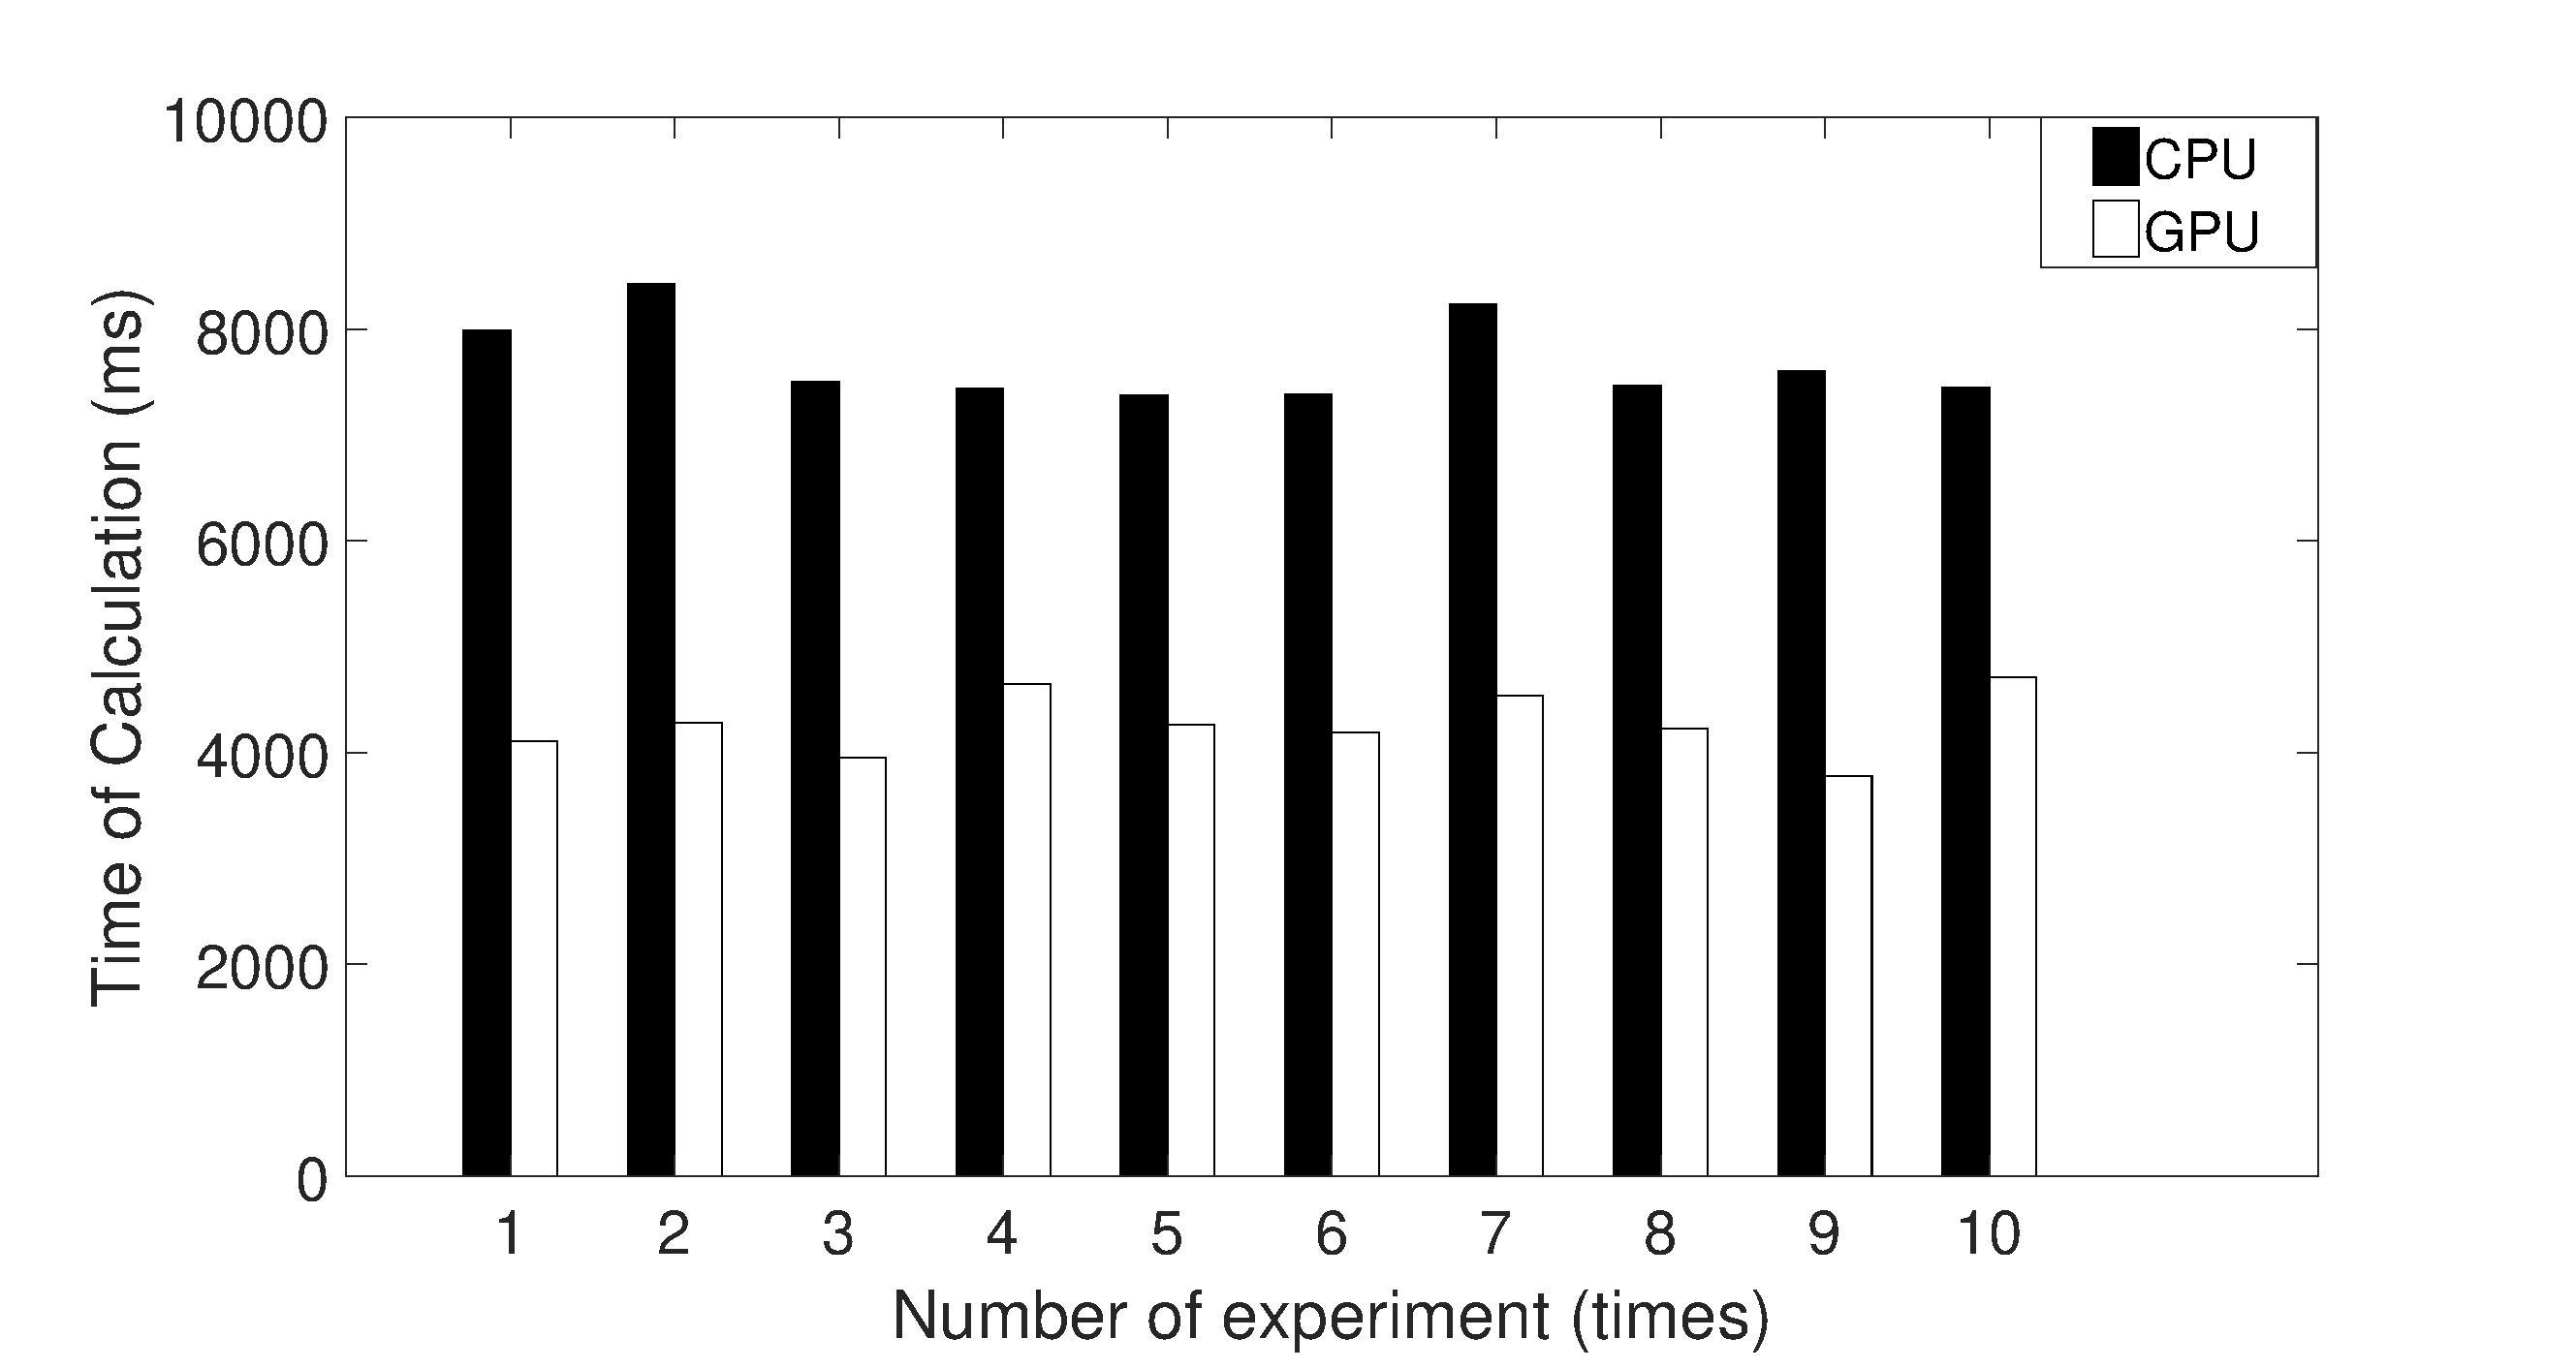
\includegraphics[width=0.8\textwidth]{figures/fig_co1.eps} }
%%   \subfigure[\projectB{}'s executing time spend on CPU is \emph{2.10} times than GPU]{
%%     \label{fig:co:b}
%%     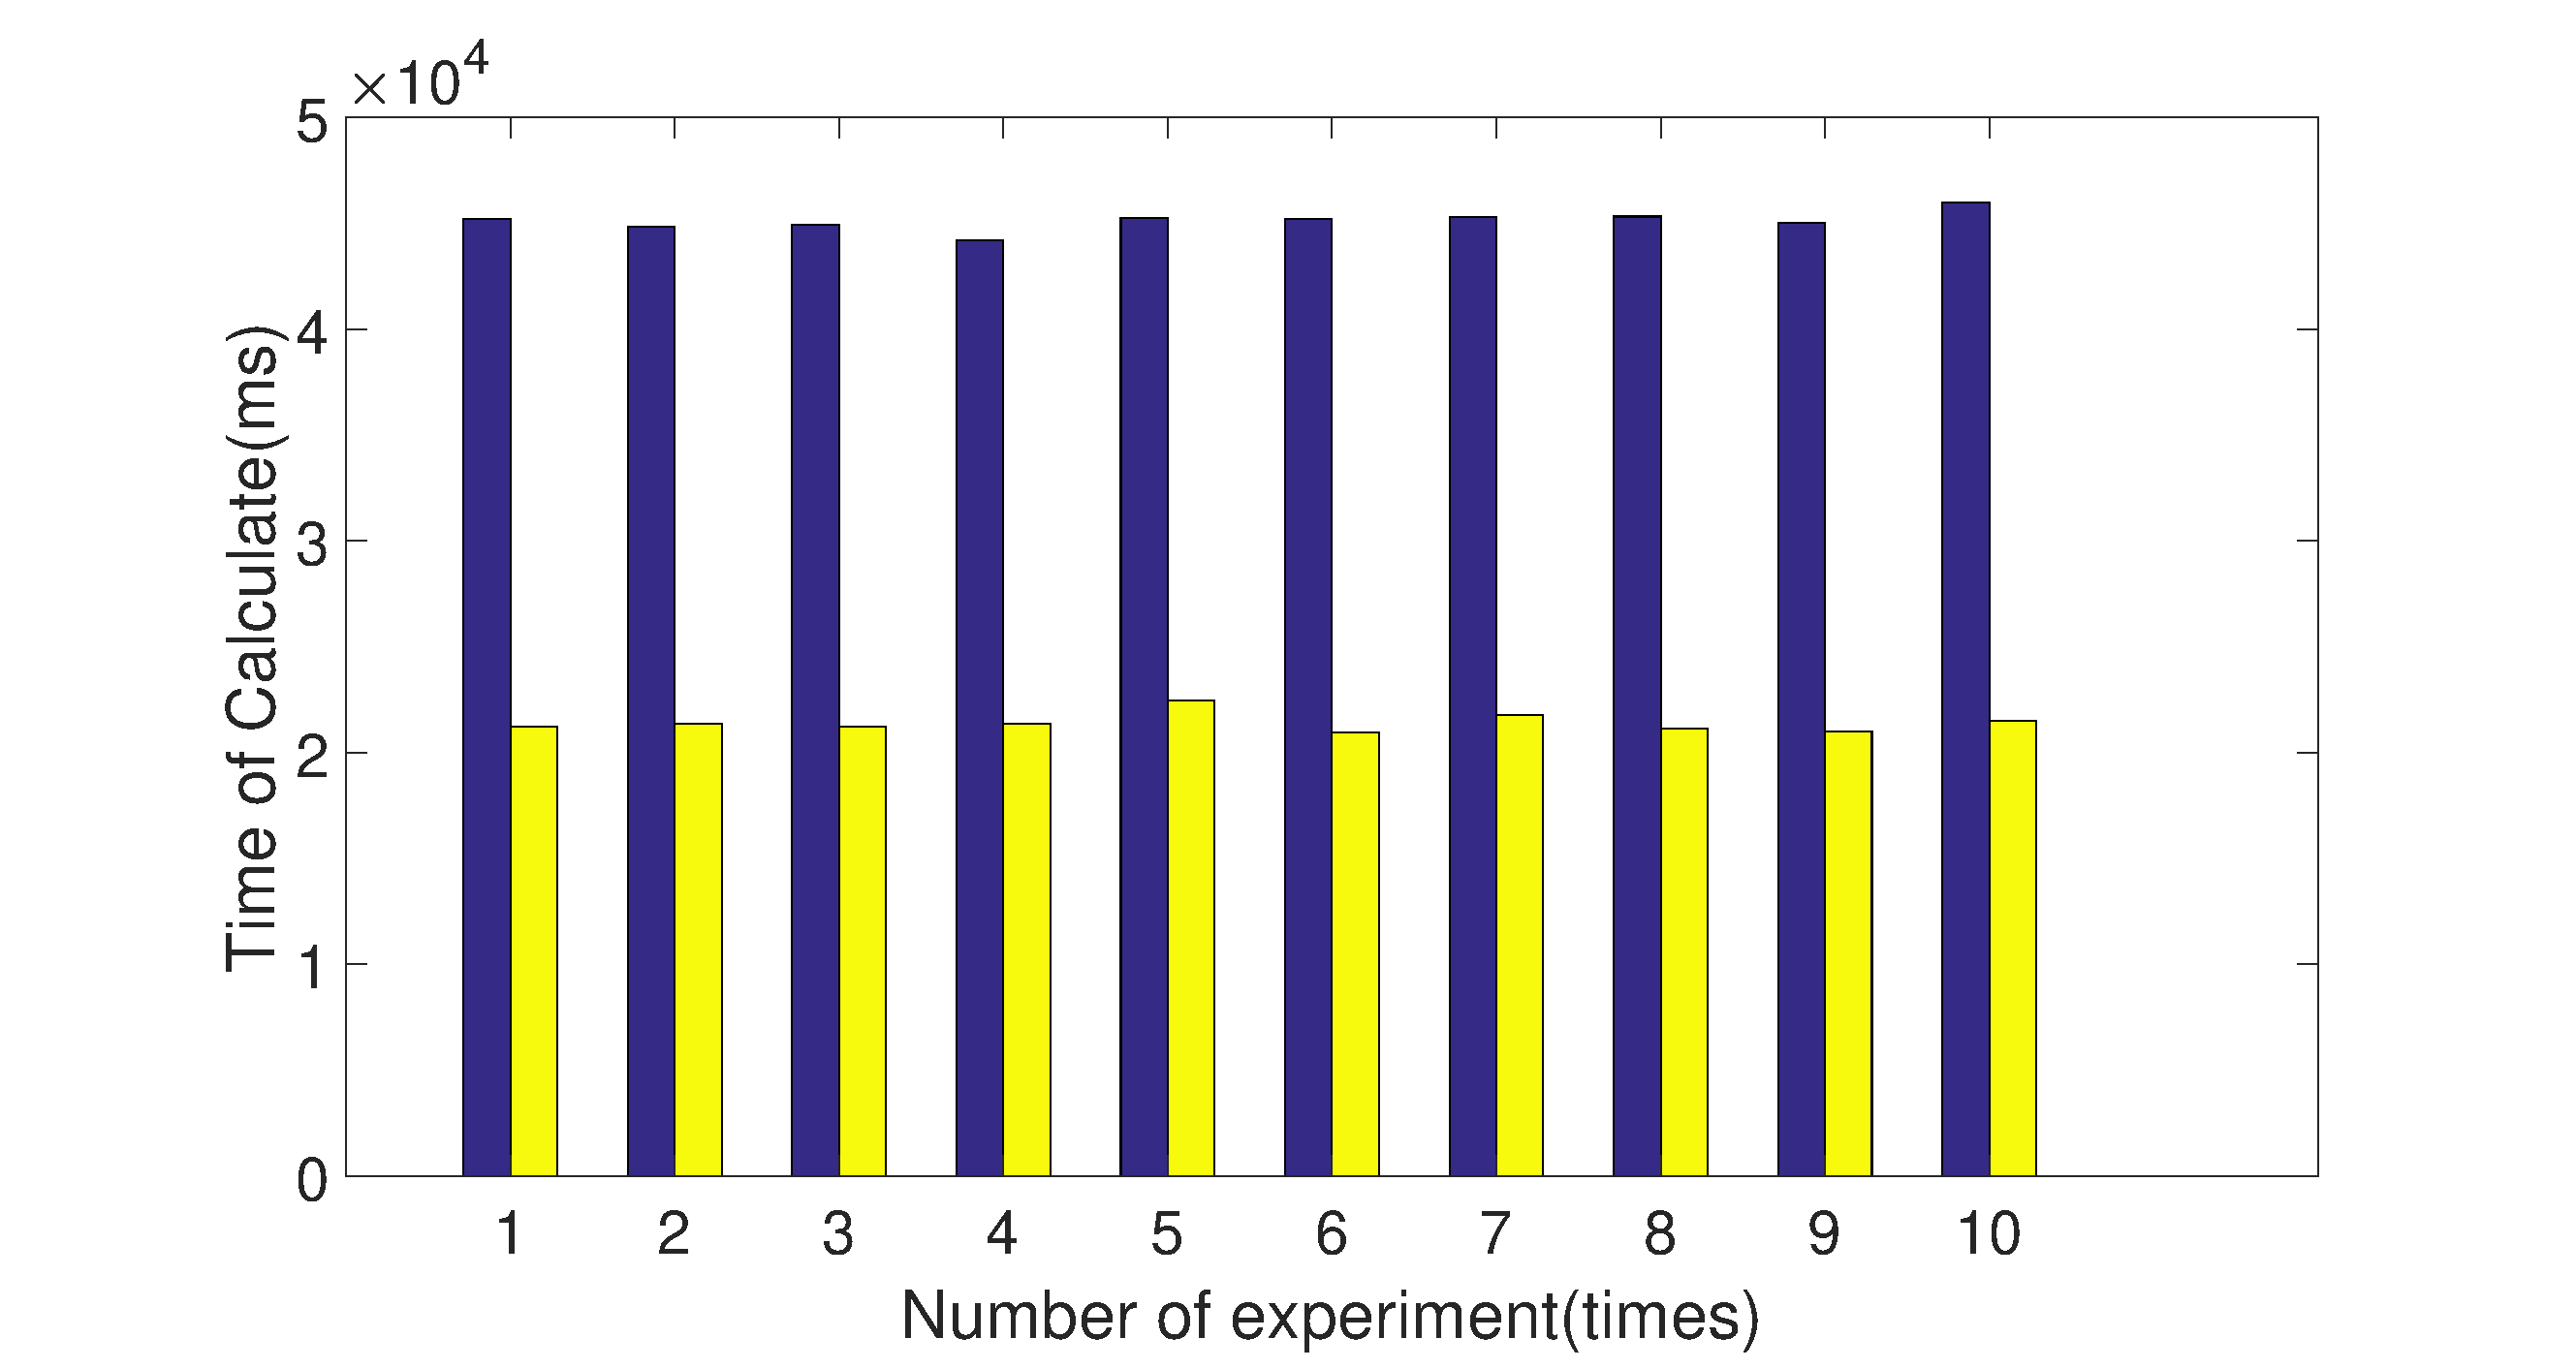
\includegraphics[width=0.8\textwidth]{figures/fig_co2.eps} }
%%   \subfigure[\projectC{}'s Executing Time on CPU is \emph{2.00} times than that on GPU]{
%%     \label{fig:co:c}
%%     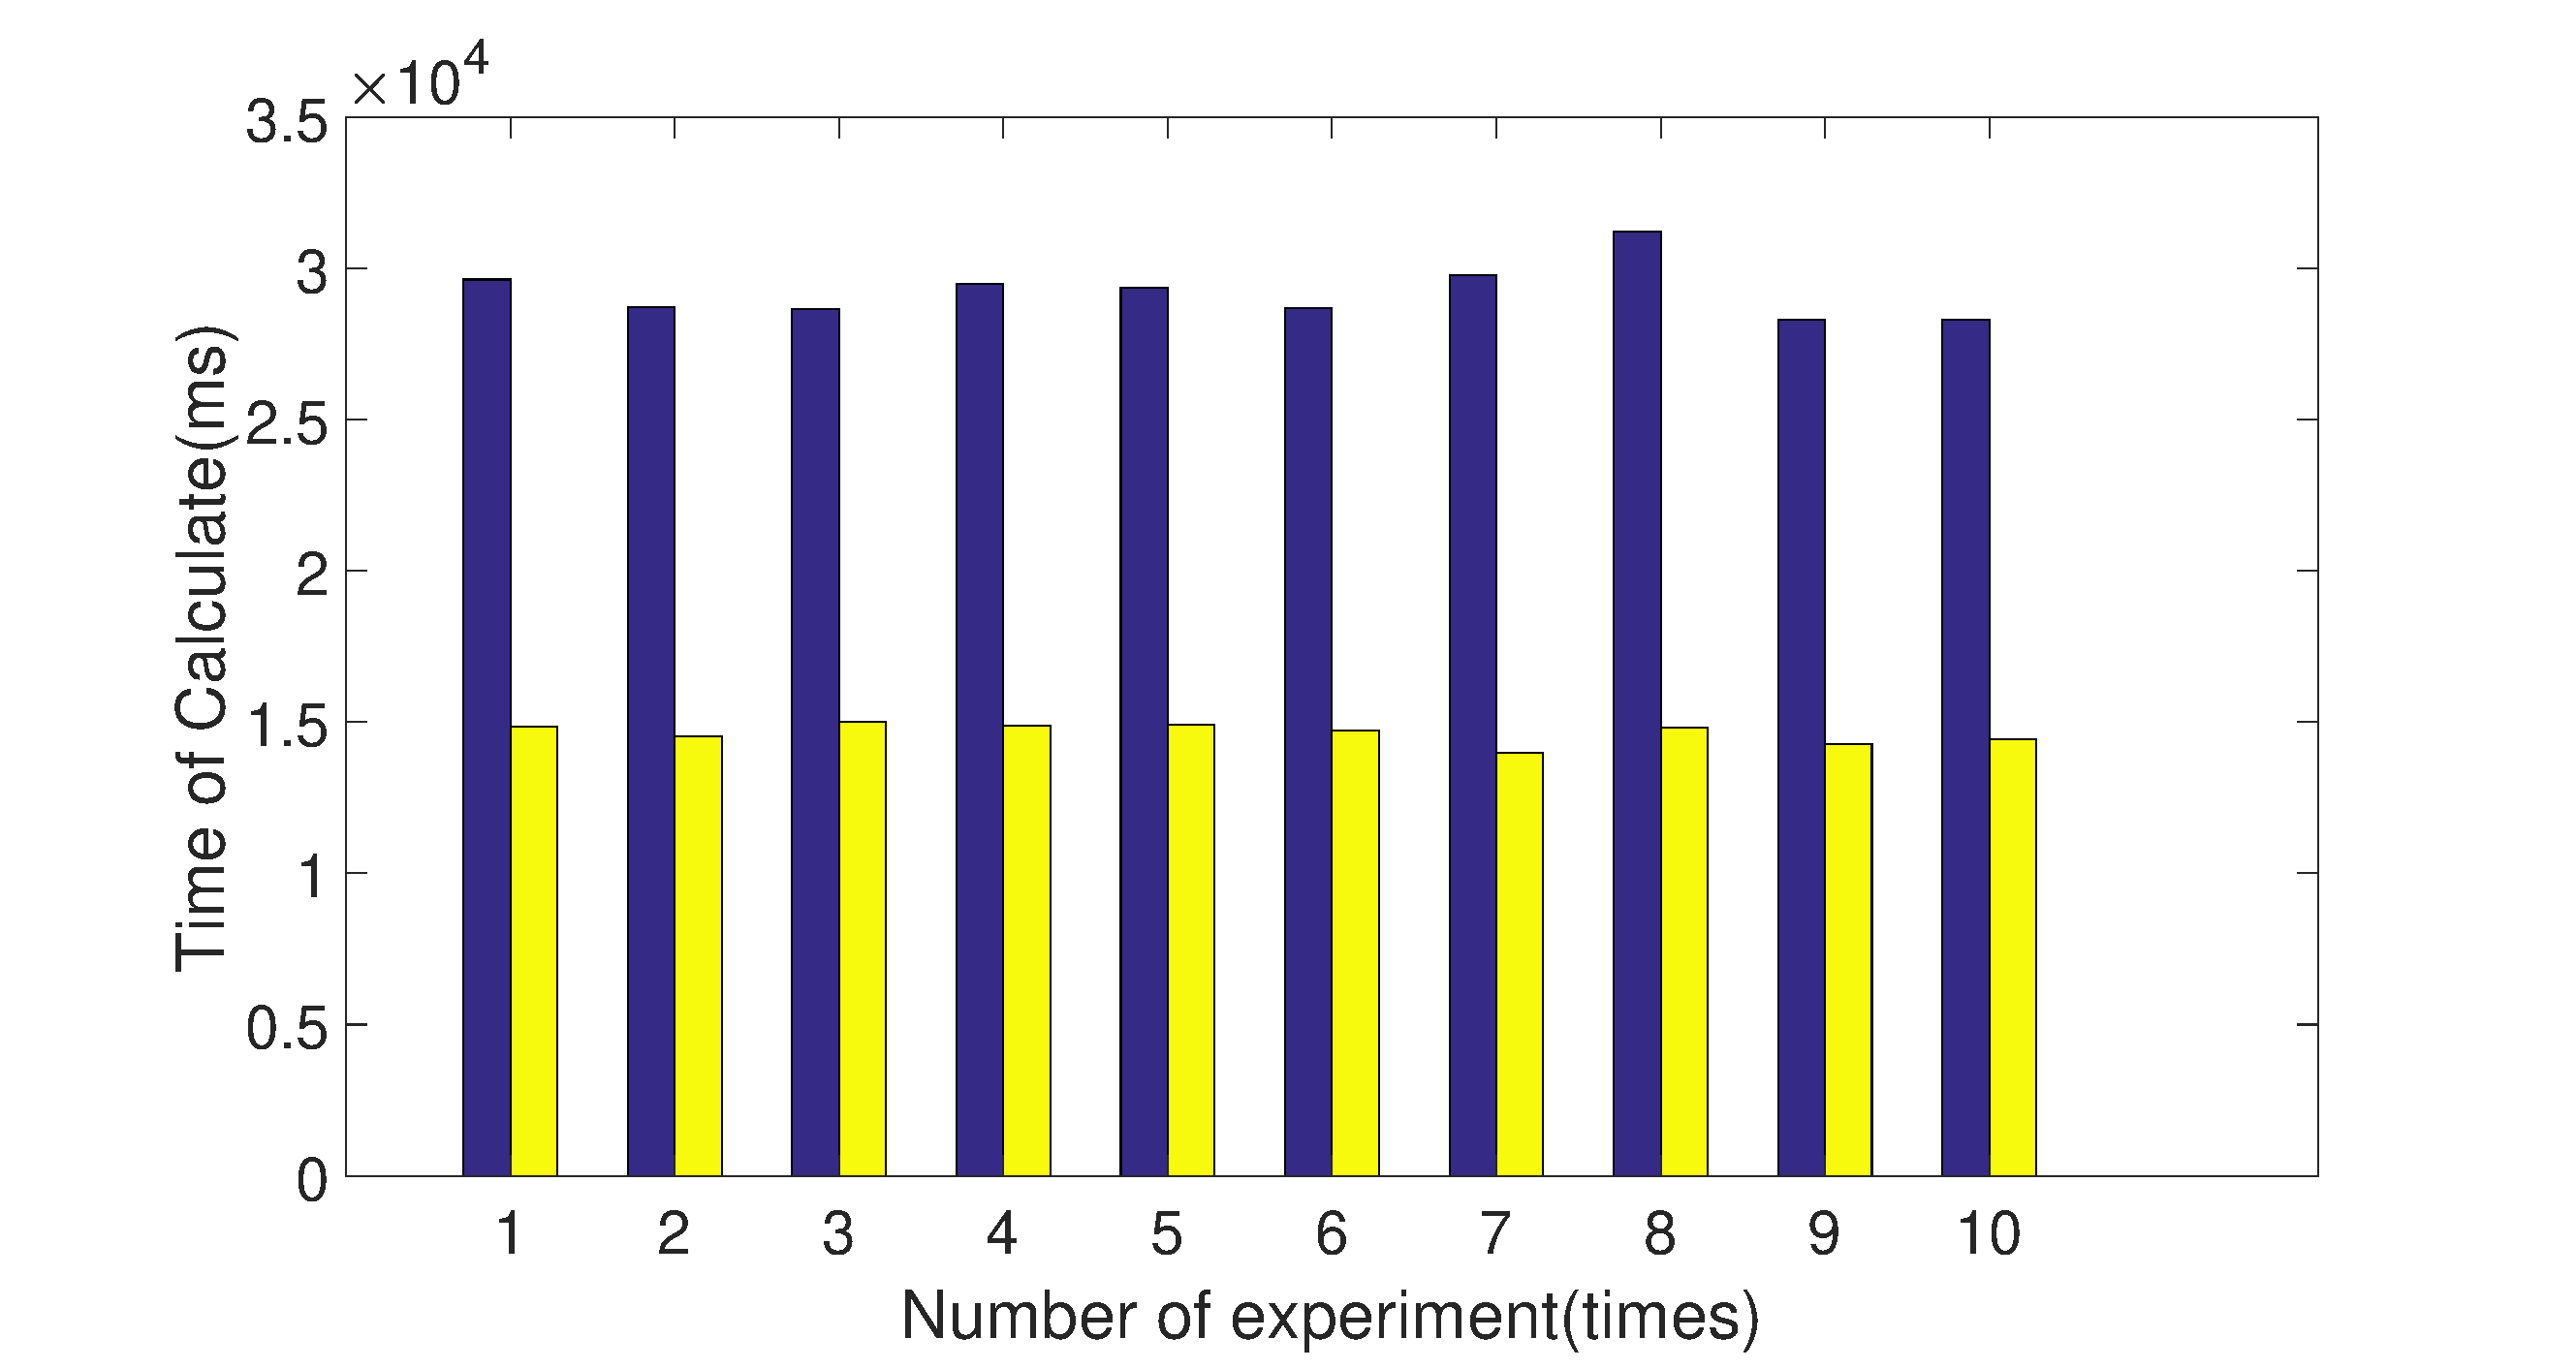
\includegraphics[width=0.8\textwidth]{figures/fig_co3.eps}
%%   }
%%   \caption{Executing Time Comparison of \emph{CPU} and \emph{GPU} Implementation}
%%   \label{fig:co}
%% \end{figure}



